%%%%%%%%%%%%%%%%%%%%%%%%%%%%%%%%%%%%%%%%%%%%%%%%%%%%%%%%%%%%%%%%%%%%%%%%%%%%%
%%%% Preamble
%%%%%%%%%%%%%%%%%%%%%%%%%%%%%%%%%%%%%%%%%%%%%%%%%%%%%%%%%%%%%%%%%%%%%%%%%%%%%

%%%% The uwthesis.sty file relies on the memoir class!
%%%% You should be using the memoir class anyway; it makes life easier:
%%%% http://www.ctan.org/tex-archive/macros/latex/contrib/memoir/
\documentclass[oneside, letterpaper, 12pt, oldfontcommands]{memoir}

%%%% Import uwthesis.sty to get official formatting, then set your variables.
\usepackage{uwthesis}
\usepackage{hyperref}
\usepackage{cite}
\usepackage{graphicx}
\newcommand{\fbinv}{\ensuremath{fb^{-1}}}

\newcommand{\PZ}{\ensuremath{Z}}
\newcommand{\Pgamma}{\ensuremath{\gamma}}
\newcommand{\Pn}{\ensuremath{\nu}}
\newcommand{\Pan}{\ensuremath{\bar{\Pn}}}
\newcommand{\zinvg}{\ensuremath{\PZ(\Pn\Pan)\Pgamma}}

\newcommand{\PW}{\ensuremath{W}}
\newcommand{\PWplus}{\ensuremath{W^\mathrm{+}}}
\newcommand{\PWminus}{\ensuremath{W^\mathrm{-}}}
\newcommand{\PWone}{\ensuremath{W^{1}}}
\newcommand{\PWtwo}{\ensuremath{W^{2}}}
\newcommand{\PWthree}{\ensuremath{W^{3}}}
\newcommand{\PB}{\ensuremath{B}}
\newcommand{\Pg}{\ensuremath{g}}
\newcommand{\PH}{\ensuremath{H}}
\newcommand{\Pp}{\ensuremath{p}}
\newcommand{\Pq}{\ensuremath{q}}
\newcommand{\Paq}{\ensuremath{\bar{q}}}
\newcommand{\Pu}{\ensuremath{u}}
\newcommand{\Pd}{\ensuremath{d}}
\newcommand{\Pc}{\ensuremath{c}}
\newcommand{\Ps}{\ensuremath{s}}
\newcommand{\Pt}{\ensuremath{t}}
\newcommand{\Pb}{\ensuremath{b}}
\newcommand{\Pe}{\ensuremath{e}}
\newcommand{\Pmu}{\ensuremath{\mu}}
\newcommand{\Ptau}{\ensuremath{\tau}}
\newcommand{\Pne}{\ensuremath{\Pn_\mathrm{e}}}
\newcommand{\Pnmu}{\ensuremath{\Pn_\mathrm{\mu}}}
\newcommand{\Pntau}{\ensuremath{\Pn_\mathrm{\tau}}}

\newcommand{\pT}{\ensuremath{p_\mathrm{T}}}
\newcommand{\vecpT}{\ensuremath{\vec{p}_\mathrm{T}}}
\newcommand{\ET}{\ensuremath{E_\mathrm{T}}}
\newcommand{\ETgamma}{\ensuremath{E_\mathrm{T}^{\gamma}}}
\newcommand{\MT}{\ensuremath{M_\mathrm{T}}}
\newcommand{\MET}{\ensuremath{p_\mathrm{T}^\mathrm{miss}}}
\newcommand{\vecMET}{\ensuremath{\vec{p}_\mathrm{T}^\mathrm{miss}}}

% Hyphenation of uncommon terms
\hyphenation{cal-ori-me-ter}
\hyphenation{cal-ori-me-ters}

\setsecnumdepth{subsection}

\settitle{A Measurement of \zinvg\ Production and a Search for New Physics in
Monophoton Events Using the CMS Detector at the LHC}
\setauthor{James Joseph Buchanan}
\setdepartment{Physics}
\doctors % or \masters
\setgraddate{2018}
\setdefensedate{T.B.D.} % or whatever format you want

%%%% Members of the Final Oral Committee (FOC)
%%%% Give name, rank, and department
%%%% 
\setfoca{Sridhara Dasu}{Professor}{Physics} % <- Your advisor
\setfocb{Wesley Smith}{Emeritus Professor}{Physics}
\setfocc{Matt Herndon}{Professor}{Physics}
\setfocd{T.B.D.}{Professor}{Physics}
\setfoce{T.B.D.}{Professor}{Something Else}
% \setfocf{Grover Cleveland}{Professor}{Zoology}

%%%% Your abstract, used for the UMI abstract and in your front matter
\setabstract{%
  This thesis presents several studies of monophoton final states
  using 35.9 \fbinv\ of 13 TeV proton-proton collision data collected by the CMS
  experiment at the LHC in 2016. The standard model \zinvg\ cross section is measured
  as a function of photon transverse momentum. No significant deviations from standard
  model predictions are observed.
  The results are also interpreted in the context of several new physics models.
  Limits are placed on coupling strengths of anomalous triple gauge couplings between
  photons and \PZ\ bosons,
  new particle masses in simplified models of dark matter, the suppression scale of a dark matter
  effective field theory model, and the graviton mass scale in a model of extra
  spatial dimensions.
}

%%%%%%%%%%%%%%%%%%%%%%%%%%%%%%%%%%%%%%%%%%%%%%%%%%%%%%%%%%%%%%%%%%%%%%%%%%%%%
%%%% Document
%%%%%%%%%%%%%%%%%%%%%%%%%%%%%%%%%%%%%%%%%%%%%%%%%%%%%%%%%%%%%%%%%%%%%%%%%%%%%

\begin{document}

% Tell the memoir class to set up lowercase roman for pagination, etc.
\frontmatter

%%%% Uncomment this to create a UMI abstract page.
%%%% If you are submitting electronically, however, this page is unnecessary.
% \theumiabstract

% The title page
\thetitlepage
\clearpage

% The copyright page, if you want to pay the fee and register copyright.
\thecopyrightpage
\cleardoublepage

% These above pages should not be counted, so we reset the counter to 1.
\setcounter{page}{1}

% An abstract may be required by your department.
\section{Abstract}
\uwabstract
\cleardoublepage

% Acknowledgements go here if you want to include them.
\section{Acknowledgements}
Acknowledgements go here.
\clearpage

% Table of contents
\maxtocdepth{subsection}
\tableofcontents* % the * means that there isn't an entry for the TOC itself
\clearpage
\listoffigures  % if you have any figures
% \clearpage
% \listoftables   % if you have any tables

% Tell the memoir class to set up normal pagination, etc. for the main doc
\mainmatter

\chapter{Introduction} \label{chap:introduction}
\section{Overview} \label{sec:introduction_overview}
This thesis presents several analyses of event
yields in ``monophoton'' final states, characterized by a single \Pgamma\ with high transverse
momentum, along with an overall transverse momentum imbalance typically of equal magnitude and opposite direction to
that of the photon.
These analyses correspond to 35.9 \fbinv\ of 13 TeV proton-proton (\Pp\Pp) collision data collected in 2016 by the CMS
detector at the LHC. A measurement of the production rate for the process $\Pp\Pp \to \PZ\Pgamma \to \Pn\Pan\Pgamma$ is obtained
and compared to predictions derived from the standard model (SM) of particle physics. No significant deviation from SM
predictions is observed.

The predicted monophoton yield in several theories of physics beyond the SM (BSM) is higher than the SM prediction.
This thesis examines two varieties of anomalous triple gauge coupling (aTGC), simplified models of dark matter (DM)
interacting with SM matter via a vector or axial-vector mediator, an effective field theory (EFT) of DM interaction
with  \Pgamma\ and \PZ\ bosons, and a model of extra spatial dimensions. For each of these models, 95\% confidence level (CL)
limits are placed on relevant parameters based on the observed collision data.

\section{Standard model of particle physics} \label{sec:introduction_standard_model}
The ``standard model'' of particle physics is our current best mathematical framework for describing the behavior
of elementary particles. The set of particles described by the SM is illustrated in Fig.~\ref{fig:sm_particles}, which
groups them according to certain fundamental characteristics.
Each particle has an intrinsic angular momentum known as spin, specified by the lower number in each square of Fig.~\ref{fig:sm_particles}.
Spin can be an integer or half-integer, according to which the particle is classified as a boson or fermion, respectively.
The fundamental fermions comprise six ``flavors'' of quarks (\Pu, \Pd, \Pc, \Ps, \Pt, \Pb) and six flavors of leptons
(\Pe, \Pmu, \Ptau, along with three corresponding neutrinos \Pne, \Pnmu, \Pntau),
each of which has both a particle and an anti-particle variety; the quarks additionally come in three ``colors''.
We denote a particle by a letter, e.g. $q$ for a generic quark; its antiparticle partner has an overbar, e.g. $\bar{q}$.
The fundamental bosons comprise the \PH\ as well as the gauge bosons, in turn comprising the \PZ, photon (\Pgamma),
two \PW s distinguished by their electric charge, and eight gluons (\Pg) distinguished by a color-anticolor doublet.

\begin{figure}[hbtp]
  \begin{center}
    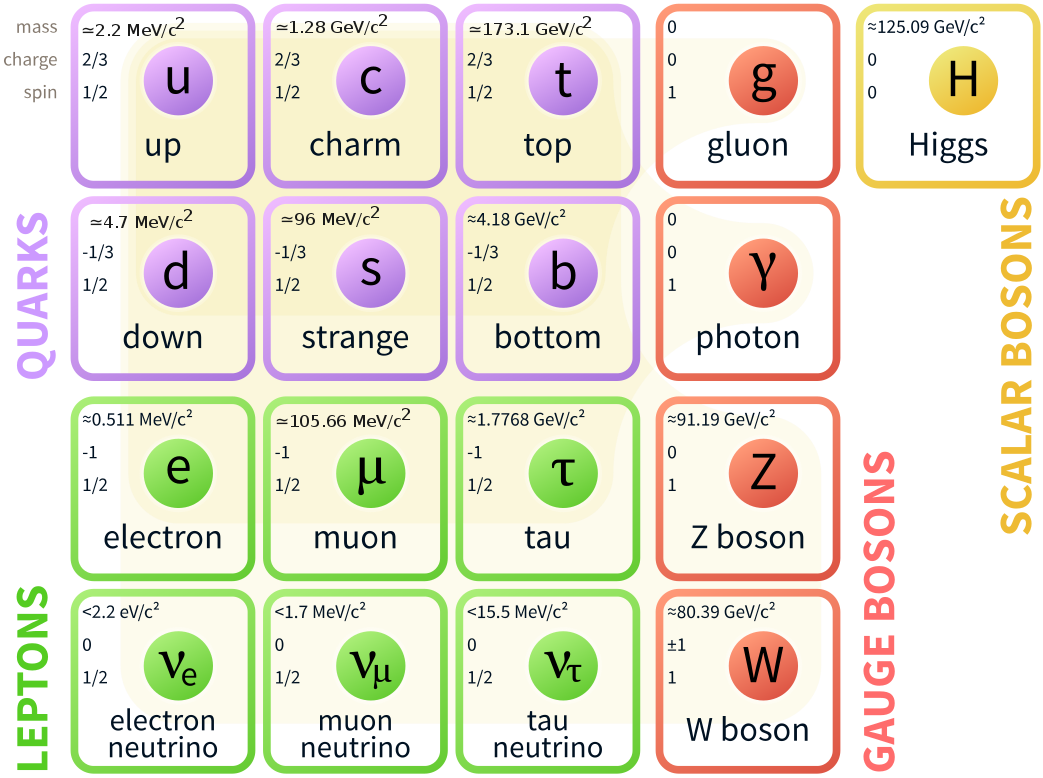
\includegraphics[width=1.0\textwidth]{Figures/sm_particles.png}
    \caption{
      The particles of the Standard Model.
    }
    \label{fig:sm_particles}
  \end{center}
\end{figure}

The particles are related to one another through various
classes of interactions, each of which has a corresponding charge whose sum must be conserved in any physical process.
The electromagnetic and weak interactions correspond to electric charge and weak isospin, respectively.
In Fig.~\ref{fig:sm_particles}, the value $Q$ of the electric charge is specified by the middle number in each square.
For quarks and leptons, weak isospin determines whether the particle is ``up-type''
(\Pu, \Pd, \Pt, \Pne, \Pnmu, \Pntau) or ``down-type'' (\Pd, \Ps, \Pb, \Pe, \Pmu, \Ptau).
Weak isospin has a corresponding value $T_{3}$: up-type fermions have $T_{3} = \mathrm{+}1/2$, down-type fermions and the \PH\ have
$T_{3} = \mathrm{-}1/2$, $W^\pm$ have $T_{3} = \pm1$, and the other bosons have $T_{3} = 0$.
The three colors carried by quarks and gluons are associated with a third interaction, described by the theory of quantum
chromodynamics (QCD). The preceding discussion applies to normal (i.e. not anti-) particles; antiparticles carry opposite values of all the
aforementioned charges.

These interactions lead to the relationships illustrated in Fig.~\ref{fig:sm_interactions}, in which every linkage represents
a direct ``coupling'', which allows a particle at one end of the link to evolve directly into a particle at the other end.
Particles with a nonzero electric charge are all coupled directly to the photon. The photon is coupled to the weak bosons
(\PZ\ and \PW), which in turn couple to all of the fundamental fermions.
The gluons couple directly with each other and with the quarks.
Particles that couple directly to the \PH\ have an intrinsic mass (specified by the top number in each square of Fig.~\ref{fig:sm_particles})
tied to the strength of their coupling. In the SM, any particle that does not couple directly to the \PH\ is massless.

\begin{figure}[hbtp]
  \begin{center}
    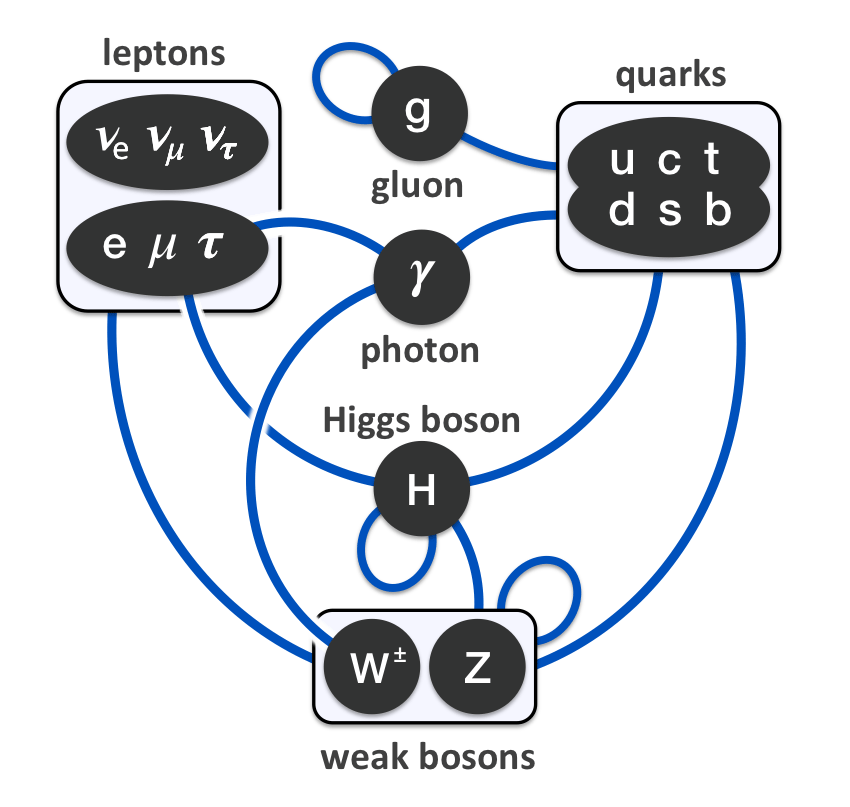
\includegraphics[width=0.7\textwidth]{Figures/Elementary_particle_interactions_in_the_Standard_Model.png}
    \caption{
      Standard Model couplings.
    }
    \label{fig:sm_interactions}
  \end{center}
\end{figure}

The full dynamics of the SM is encapsulated mathematically by a Lagrangian function. Particles correspond to operator
terms appearing in the Lagrangian, and a coupling of one particle to another is described by multiplying their
corresponding operators together. The SM Lagrangian is unchanged
if all its fermion operators are multiplied by any complex number of the form $e^{iY\theta}$, where $Y$ is a value that depends
on the operator being multiplied. The is true even if $\theta$ is allowed to have different arbitrary values at
different points in space and time, but any operator with a nonzero $Y$ couples to the \PB, and as a consequence the first derivatives
of $\theta$ in space and time must also be subtracted from \PB.
This deep level of invariance is called a gauge symmetry, with \PB\ the associated gauge boson.
Multiplication by $e^{i\theta}$ is characterized by the group $U(1)$, so we say that the SM Lagrangian has a
$U(1)_{Y}$ gauge symmetry associated with the \PB.

In a similar vein, the SM Lagrangian is unchanged if matching doublets
of weak isospin up- and down-type operators are multiplied by unitary $2\times2$ matrices with determinant 1, described by the
group $SU(2)$. Those with a nonzero weak isospin couple to every $W^{i}$ ($i=1,2,3$), which must receive their own balancing transformations
if the fermion $SU(2)$ transformations are allowed to vary as a function of space and time.
Hence we say that the SM Lagrangian has an $SU(2)$ gauge symmetry associated with the gauge bosons $W^{i}$.

The \PB\ and $W^{i}$s also couple to the \PH, and the structure of this coupling constrains the physical states
most easily accessed by these operators, corresponding to four distinct linear combinations of
\PB\ and $W^{i}$. These combinations, which are themselves operators, are labeled \PZ, \Pgamma, \PWplus, and \PWminus,
and these are the operators describing the physical particles detected in experiments.
In this manner, the electromagnetic and weak interactions are intertwined in what is known as the electroweak (EWK) interaction.
The conserved electric charge $Q$ emerges as the sum of $T_{3}$ with $\frac{1}{2}Y$.

Finally, the SM Lagrangian has an additional $SU(3)$ gauge symmetry associated with the eight gluons and color charge, described by QCD.
Particles with color charge do not exist stably on their own, but rather are always observed in bound states called hadrons, in which the total color
charge of the bound state is invariant under any $SU(3)$ transformation. One such ``colorless'' configuration is the proton (p), which
to a first approximation may be thought of as a bound state of two $u$ quarks and one $d$ quark. However, the mass of the proton is
much greater than the sum of the masses of these three components, and this additional mass is associated with an effervescent ``sea''
of partons, transient particles swarming the proton that can only be distinguished at high energies. Known partons include
all types of quark and antiquark. As a consequence, a high-energy collision between two protons can give rise to a $q\bar{q}$ interaction,
the primary catalyst for all the processes studied below. A single parton carries some fraction of the total energy carried by the whole proton,
so in general, partons collide with a lower interaction energy than that of the protons that carry them.
The square of the center-of-mass energy of colliding protons is denoted by $s$, while the square of the center-of-mass energy of a specific
parton-parton interaction is denoted $\hat{s}$.

This rapid overview of the SM necessarily elides many essential nuances of the underlying mathematical formalism. These are more fully
documented in numerous comprehensive texts on the subject, e.g.~\cite{ref:HalzenMartin, ref:BargerPhillips, ref:PeskinSchroeder, ref:Srednicki, ref:Schwartz}.
The SM does not describe every observed physical phenomenon: for example, it does not describe DM (the subject of sec.~\ref{sec:introduction_dm})
or gravitation (the subject of sec.~\ref{sec:introduction_ADD}). Its domain of applicability is nevertheless quite substantial, encompassing
every well-measured fundamental interaction of every verified fundamental particle, and after decades of precision studies, no significant deviation from
its predictions has ever been confirmed within this domain~\cite{ref:PDG}.

\section{\texorpdfstring{\zinvg}{Z(νν)γ} cross section} \label{sec:introduction_znng}
In a collision of two beams of particles, the average rate of any specific collision process is directly proportional to the
number of particles in each of the colliding beams, to their density in the plane transverse to the beam direction, and to the average
frequency at which particles are made to come into contact. These three features determine the instantaneous luminosity $L$ of a pair
of colliding beams, and the overall average rate of a given process may be written as $\sigma L$, where $\sigma$
is a constant of proportionality. Since $\sigma$ has dimensions of area, it is called the cross section.

Cross sections may be calculated using Feynman diagrams. These are
assembled by combining fundamental interaction vertices: the SM vertices relating the fermions and gauge bosons are listed in Fig.~\ref{fig:sm_vertices}.
Mathematical terms are assigned to Feynman diagrams according to a prescription known as the Feynman rules, which can be derived from the Lagrangian.
This process results in a mathematical expression $\mathcal{M}_{i}$ for each diagram $i$ one wishes to consider. The cross section is the sum of $|\sum_{i}{\mathcal{M}_{i}}|^{2}\rho$
over all kinematically consistent initial and final states of the given process ($\rho$ depends on the allowed kinematic parameters and is called the phase space
factor). This method for calculating cross sections using Feynman diagrams is more fully described in Refs.~\cite{ref:HalzenMartin, ref:BargerPhillips};
a development in the context of quantum field theory is given in Refs.~\cite{ref:PeskinSchroeder, ref:Srednicki, ref:Schwartz}.

\begin{figure}[hbtp]
  \begin{center}
    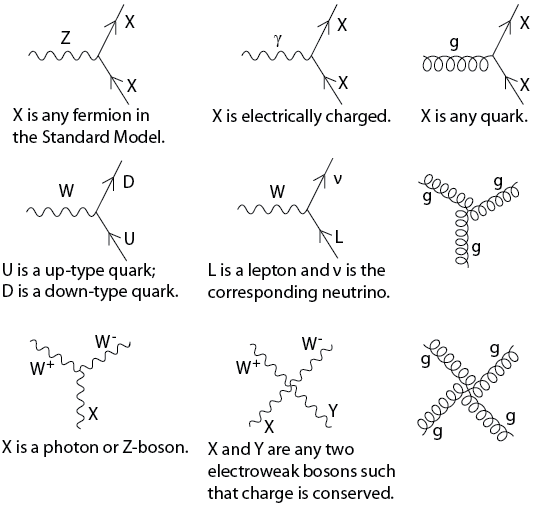
\includegraphics[width=0.7\textwidth]{Figures/Standard_Model_Feynman_Diagram_Vertices.png}
    \caption{
      Fermion and gauge boson vertices of the standard model.
    }
    \label{fig:sm_vertices}
  \end{center}
\end{figure}

The Feynman rule for a vertex includes a numerical factor $g$. These are typically less than 1 in high-energy collisions, and therefore diagrams
with additional vertices make smaller contributions to a cross section calculation.
The expression $|\sum_{i}{\mathcal{M}_{i}}|^{2}$ can therefore be organized as a sum of terms with increasing powers of $\alpha \propto g^{2}$, which make successively smaller
contributions to the cross section.
Terms with the lowest powers of $\alpha$ are called leading order (LO) terms, followed by next-to-leading order (NLO), next-to-next-to-leading order (NNLO), etc.
Diagrams with an internal loop contain at least one more vertex than equivalent diagrams without the loop, and therefore diagrams without any internal loops,
called tree-level diagrams, make the only contributions at LO. Each class of interaction has its own characterisitc $\alpha$: for example, QCD is characterized by $\alpha_\mathrm{S}$.

In the SM, events with a monophoton signature arise at the LHC (Chap.~\ref{chap:LHCCMS}) primarily from the process $pp \to \PZ\Pgamma \to \Pn\Pan\Pgamma$,
where $q$ is any single species of quark, \Pn\ is any single species of neutrino, and the neutrino-antineutrino pair arises from the decay
of a short-lived \PZ\ boson. The leading tree-level diagram for this process is shown in Fig.~\ref{fig:zinvg_diagrams}(a). We typically abbreviate this process by
reference to its final state, \zinvg. The final-state photon can be detected, but the neutrinos only interact with SM particles via the mediation
of \PZ\ and \PW\ bosons, and these interactions are strongly suppressed by the high masses of those particles. Hence, neutrinos almost never interact directly with the LHC's detectors.

\begin{figure}[htb]
  \begin{center}
    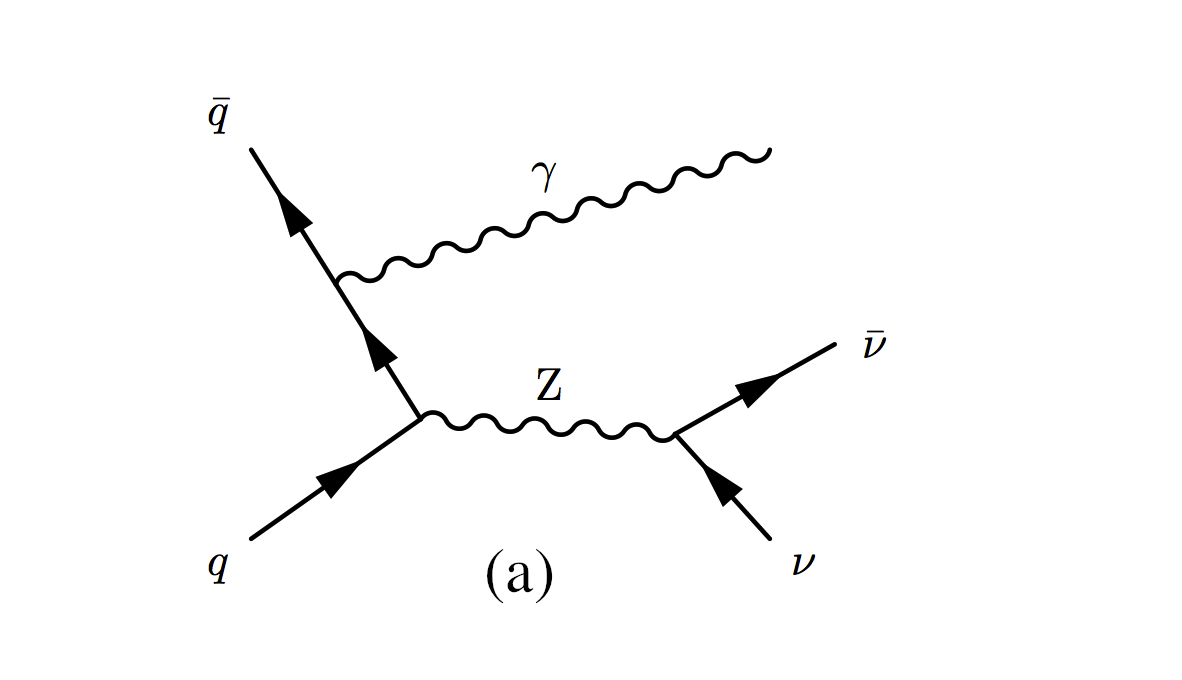
\includegraphics[width=0.49\textwidth]{Figures/zg_isr_v11.pdf}
    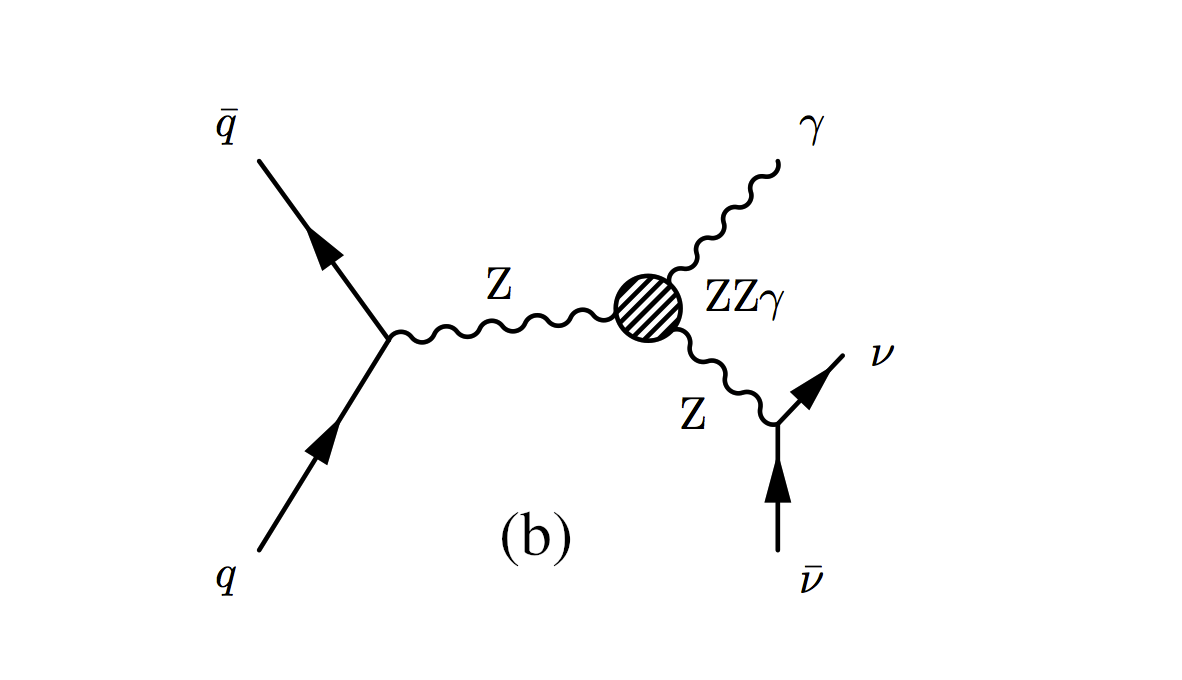
\includegraphics[width=0.49\textwidth]{Figures/zg_zzg_v11.pdf}
    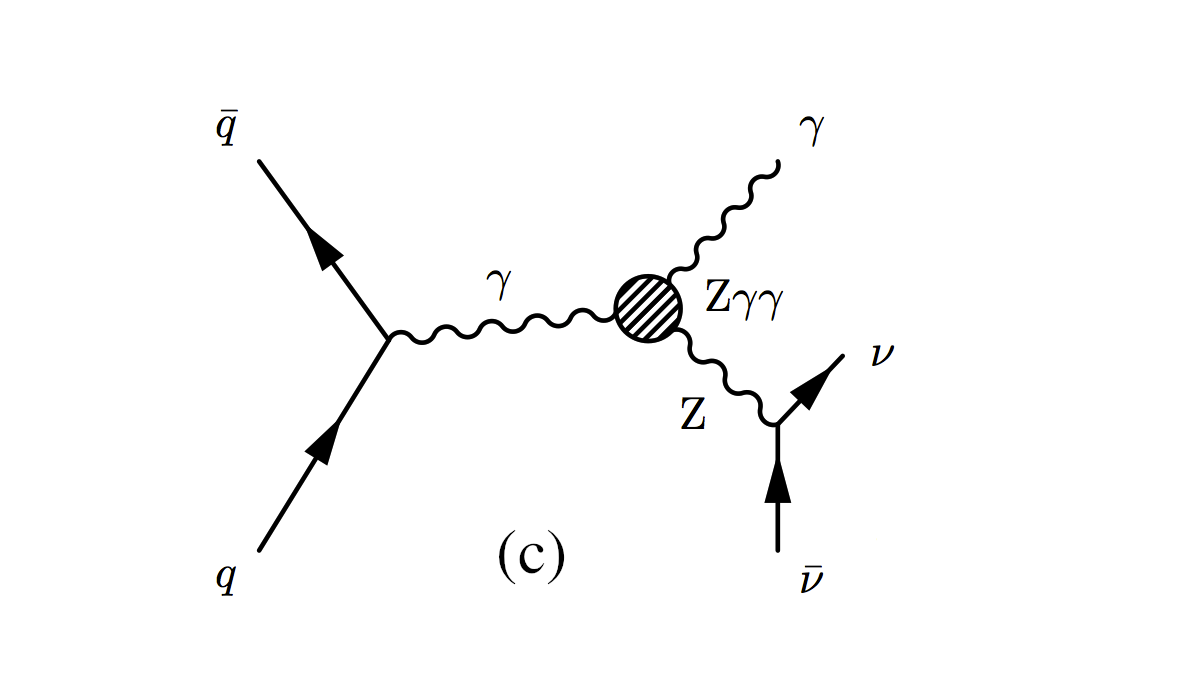
\includegraphics[width=0.49\textwidth]{Figures/zg_zgg_v11.pdf}
    \caption{
      The leading Feynman diagrams for \zinvg\ production arising from $pp$ collisions. Diagram (a) is the leading SM contribution.
      Diagrams (b) and (c) show contributions from aTGC vertices.
    }
    \label{fig:zinvg_diagrams}
  \end{center}
\end{figure}

Their existence is instead inferred by their absence.
In a collider experiment, the vectorial momentum transverse to the beam direction, \vecpT, must sum to approximately zero in the reference frame of the
detector. The negative vector sum of \vecpT\ for all detected particles in an event is denoted \vecMET, and its magnitude \MET\ must therefore be close
to zero if all the particles in an event are reliably detected and their momenta are accurately measured. The only high-momentum SM particles that can't
be reliably detected are neutrinos, so a large value of \MET\ can be a sign of neutrino production. An event with a high-\pT\ detected photon, in which
the \vecMET\ has a large magnitude and points in a direction significantly different from that of the photon, is called a monophoton event, and it is
expected that \zinvg\ processes are the main contributors of high-\pT\ monophoton events.

\subsection{Previous measurements} \label{sec:introduction_znng_previous_measurements}
The theoretical SM value for the \zinvg\ cross section has been calculated to NLO in QCD and EWK couplings~\cite{ref:JHEP04(2015)018, ref:JHEP02(2016)057}.
Events with additional radiated photons, quarks, or gluons are also included.
The \zinvg\ process receives NLO contributions from 1-loop QCD and EWK diagrams, as well as tree-level diagrams with up to one additional radiated \Pgamma, \Pq, or \Pg.
These can arise from initial-state $q\bar{q}$, $qg$, and $\bar{q}g$ (with QCD and EWK corrections at NLO), as well as $q\gamma$, $\bar{q}\gamma$ (with EWK corrections
at NLO) interactions~\cite{ref:JHEP02(2016)057}.

The calculation has also been done to NNLO in $\alpha_\mathrm{S}$ alone,
which includes contributions from tree-level diagrams with up to two extra radiated QCD partons (\Pq\ or \Pg), one-loop diagrams with up to one extra
radiated QCD parton, and two-loop corrections. The initial-state QCD parton interactions include those listed among the NLO contributions above,
as well as $gg$ interactions~\cite{ref:j.physletb.2014.02.037, ref:10.1007/JHEP07(2015)085}.
The exact values obtained from such a calculation depend on the specific initial and final states included. These are constrained by operating conditions
of the experiment one wishes to compare results with. In practice the cross section is computed for events containing a high-\pT\ final state photon falling within
the detector acceptance, a high-\pT\ final-state \Pn\Pan\ pair, and radiated QCD partons well-separated from the photon, also falling within the detector acceptance.



\section{Anomalous triple gauge couplings} \label{sec:introduction_aTGC}
Putative vertices joining three particles that are not found in the SM are known as aTGCs. For example, there is no fundamental SM vertex
joining a single \Pgamma\ to a pair of \PZ s, or a single \PZ\ to a pair of \Pgamma s. A model
describing the generic phenomenology of these aTGCs is developed in~\cite{ref:Nucl.Phys.0550-3213_87_90685-7, ref:PhysRevD.47.4889, ref:PhysRevD.62.113011}.
For an intermediate state $V = \PZ,\Pgamma$ decaying to a final state \PZ\Pgamma\ pair, this model parametrizes the effective vertex interaction $\PZ V\Pgamma$
by a set of factors $h_{i}^{V}$ ($i$ from 1 to 4). Increasing the values of these parameters significantly increases the cross section
of \zinvg\ processes, by allowing the reaction to proceed via the additional diagrams shown in Fig.~\ref{fig:zinvg_diagrams}(b),(c),
in which the aTGC vertices are covered by opaque circles.

The circle could be thought of as masking a more detailed process taking place underneath. The SM admits processes that are predicted to contribute
to this effective vertex, but all SM contributions to $h_{3,4}^{V}$ have at least one internal loop that could fit within the circle, and
further loops are required for $h_{1,2}^{V}$ contributions~\cite{ref:PhysRevD.47.4889}.
As a consequence, the SM contribution to all eight $h_{i}^{V}$ parameters is quite close to zero.
The observation of a substantial nonzero value for any $h_{i}^{V}$ would be a compelling sign of BSM physics.

The contributions to the \zinvg\ cross section coming from $h_{1,2}^{V}$ are independent of those from $h_{3,4}^{V}$ (for any V), and also nearly identical
in magnitude, so without loss of generality we only focus on scenarios for which $h_{3,4}^{V}$ are nonzero. The contributions
from $h_{i}^{\PZ}$ are largely independent of those from $h_{j}^{\Pgamma}$ (for any i,j), so these are examined separately.
However, the contributions from $h_{3}^{V}$ are substantially correlated with those from $h_{4}^{V}$ (and similarly for $h_{1,2}^{V}$), so we examine
scenarios in which $h_{3,4}^{V}$ take on assorted pairs of values, both of which may be nonzero. The theoretical relationships between these parameters
are explored in~\cite{ref:PhysRevD.47.4889}.

The neutrino decays of \PZ-bosons offer an especially good window on \PZ\PZ\Pgamma\ and \PZ\Pgamma\Pgamma\ aTGCs because the
probability of \PZ\ decays into neutrinos is roughly six times higher than that of decays into $e^\mathrm{+}e^\mathrm{-}$, and
also into $\mu^\mathrm{+}\mu^\mathrm{-}$. Furthermore, the probability of reconstructing a \zinvg\ event in a detector is typically
higher than that of a charged lepton event. As a consequence, aTGC limits derived from neutral \PZ\ decays can be several times
finer than limits derived from charged \PZ\ decays when analyzing the same $pp$ collision data sets (compare e.g.~\cite{ref:PhysRevD.89.092005} and~\cite{ref:JHEP10(2013)164},
based on 7 TeV LHC data; also Fig.~\ref{fig:lhc_8tev_atgc_1dlimits}, based on 8 TeV data).
The decays of \PZ\ into $q\bar{q}$ (and thence to hadrons) are difficult to distinguish in practice from hadronic \PW\ decays~\cite{ref:RevModPhys.89.035008}.

\subsection{Previous searches} \label{sec:introduction_aTGC_previous_searches}
The LEP collider established constraints on each of the eight the parameters $h_{i}^{V}$ in the context of the process $e^{\mathrm{+}}e^{\mathrm{-}} \to \PZ\Pgamma$.
In a statistical combination of searches perfomed by the DELPHI, L3, and OPAL experiments, examining 3 \fbinv\ of $e^{\mathrm{+}}e^{\mathrm{-}}$ collision data
for $\sqrt{s}$ ranging from 130 GeV to 209 GeV, the 95\% CL intervals of seven of the parameters contain 0, with total ranges between 0.05 and 0.10 for $h_{i}^{\Pgamma}$
and between 0.14 and 0.25 for $h_{i}^{\PZ}$; the 95\% CL interval for the remaining factor $h_{4}^{\gamma}$ spans 0.01 to 0.05~\cite{ref:j.physrep.2013.07.004}.

The LEP combined analysis assumed that all but one of the eight parameters were fixed to the SM expectation of 0 (i.e. these are 1D limits).
It was also the last major effort to obtain limits on $h_{1,2}^{V}$ independently of $h_{3,4}^{V}$,
as subsequent searches have taken the present approach of focusing on $h_{3,4}^{V}$ alone, for the reasons listed above.
Uniquely among the LEP experiments, the L3 Collaboration also placed limits on correlated pairs of parameters (2D limits), shown in Fig.~\ref{fig:L3_atgc_contours}~\cite{ref:j.physletb.2004.07.002}.

\begin{figure}[hbtp]
  \begin{center}
    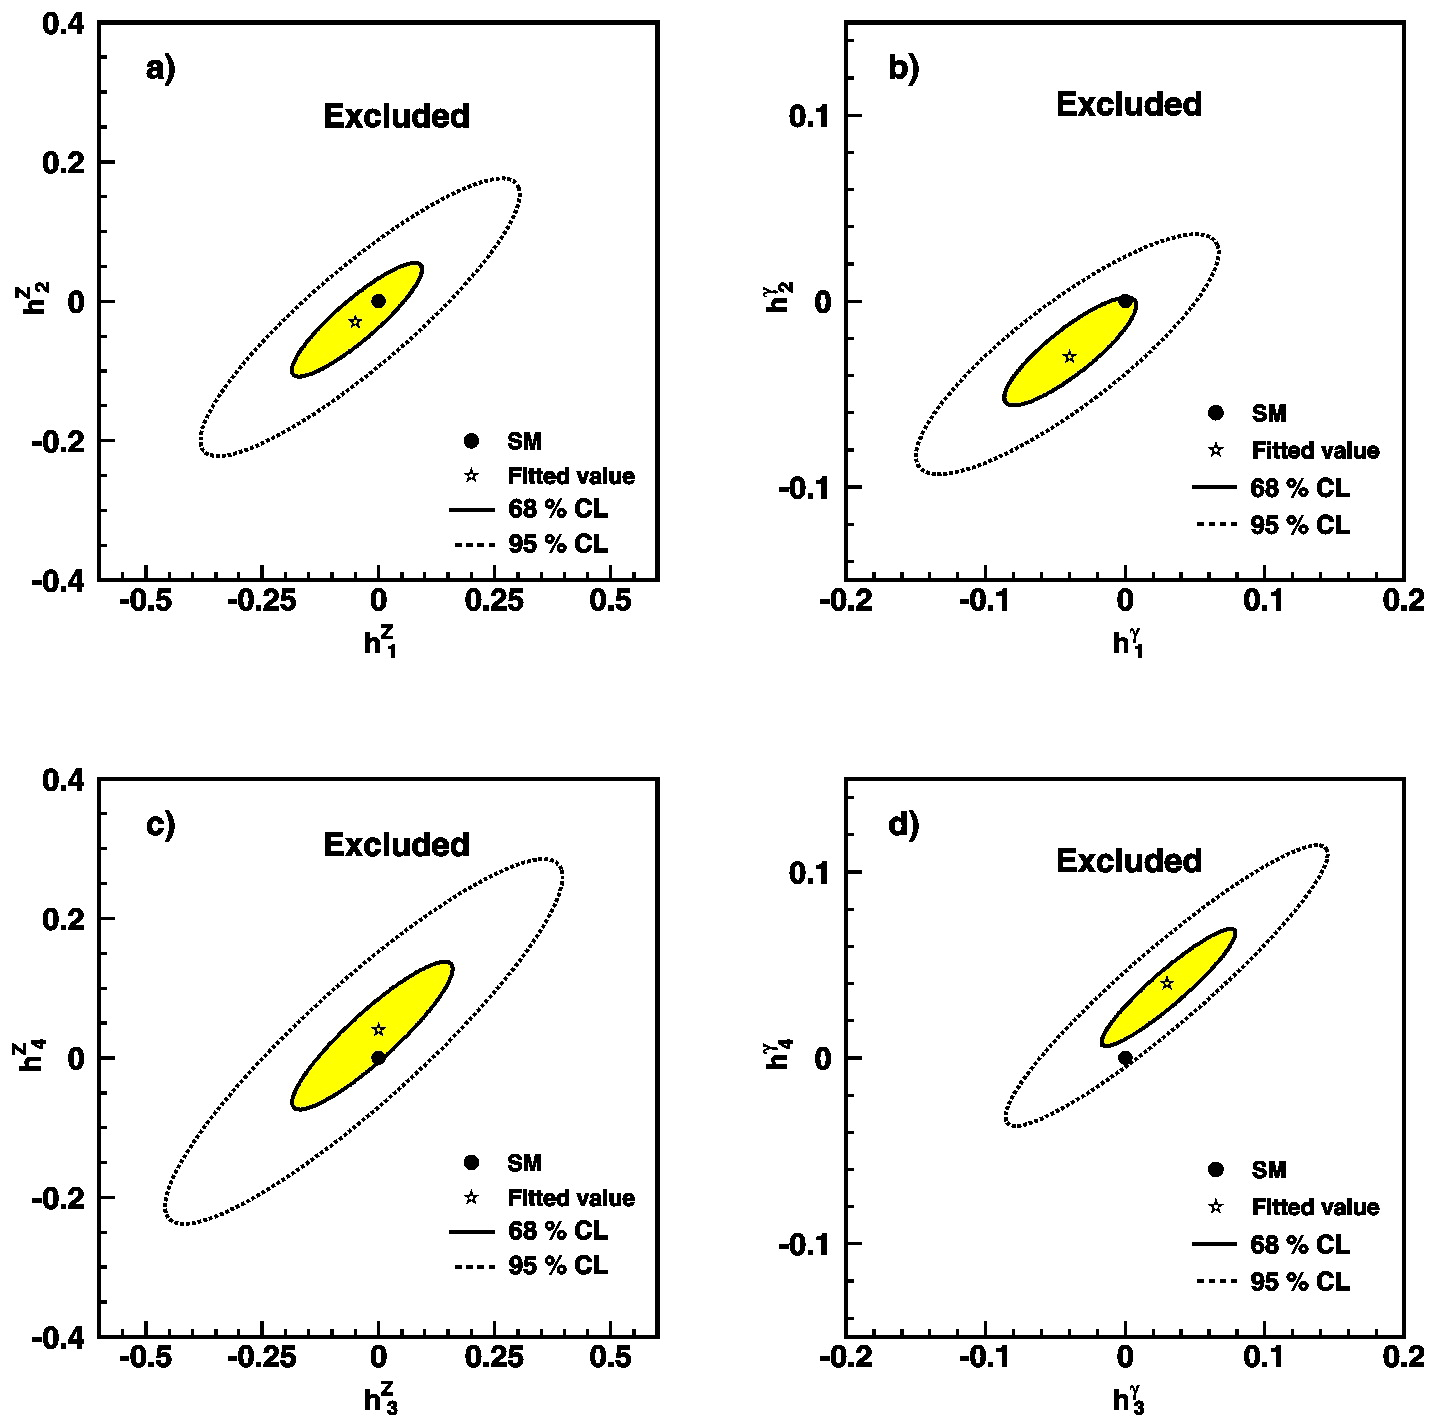
\includegraphics[width=0.8\textwidth]{Figures/L3_atgc_contours.jpg}
    \caption{
      $h_{i}^{V}$ exclusion contours from the L3 experiment at the LEP collider~\cite{ref:j.physletb.2004.07.002}.
    }
    \label{fig:L3_atgc_contours}
  \end{center}
\end{figure}

Experiments at the Tevatron collider improved these limits in analyses of $p\bar{p}$ collision data at $\sqrt{s} = 1.96$ TeV.
The Tevatron analyses incorporated a form factor $1 / (1 + \hat{s}/\Lambda^{2})^{n}$, by which a constant term $h_{0i}^{V}$ is
multiplied to obtain $h_{i}^{V}$.
The form factor is essentially arbitrary; $n$ is set equal to $i$ and $\Lambda$ (not to be confused with the EFT suppression scale, below)
is set to 1.5 TeV by convention. This form factor was introduced in the common reference~\cite{ref:PhysRevD.47.4889} but was not used in LEP~\cite{ref:j.physrep.2013.07.004}
or most subsequent LHC analyses, which treat the $h_{i}^{V}$ parameters as constants independent of $\hat{s}$.

The CDF experiment combined analyses of \zinvg\ processes, using 4.9 \fbinv\ of data, and processes where the \PZ\ decays to
$e^\mathrm{+}e^\mathrm{-}$ or $\mu^\mathrm{+}\mu^\mathrm{-}$, using 5.1 \fbinv\ of data.
They set 95\%\ Bayesian credibility intervals constraining $|h_{3}^{V}| < 0.022$ and $|h_{4}^{V}| < 0.0009$ (1D limits)~\cite{ref:PhysRevLett.107.051802}.
The D0 experiment similarly combined a 3.6 \fbinv\ \zinvg\ analysis with a 7.2
\fbinv\ $Z(e^\mathrm{+}e^\mathrm{-})\gamma$ and $Z(\mu^\mathrm{+}\mu^\mathrm{-})\gamma$ analysis to set 95\%\ CL limits constraining
$|h_{03}^{V}| < 0.027$ and $|h_{04}^{V}| < 0.0014$ (1D limits)~\cite{ref:PhysRevD.85.052001}. Correlated 2D limits were also
computed and are shown in Fig.~\ref{fig:d0_aTGC}.

\begin{figure}[hbtp]
  \begin{center}
    \includegraphics[width=0.45\textwidth]{Figures/d0_ZZg.png}
    \includegraphics[width=0.45\textwidth]{Figures/d0_Zgg.png}
    \caption{
      $h_{0i}^{V}$ exclusion contours from the D0 experiment at the Tevatron collider~\cite{ref:PhysRevD.85.052001}.
    }
    \label{fig:d0_aTGC}
  \end{center}
\end{figure}

Experiments at the LHC made further improvements via the analysis of $pp$ collision data at progressively higher $\sqrt{s}$.
A summary of 1D limits on $h_{i}^{V}$ from both the ATLAS and CMS experiments obtained from analyses of \textasciitilde20 \fbinv\ of $\sqrt{s} = 8$ TeV data
is shown in Fig.~\ref{fig:lhc_8tev_atgc_1dlimits}. ATLAS limits show the results
of combined \zinvg, $Z(e^\mathrm{+}e^\mathrm{-})\gamma$, and $Z(\mu^\mathrm{+}\mu^\mathrm{-})\gamma$
analyses, both with and without a form factor on $h_{i}^{V}$. CMS limits show separate \zinvg\ results,
along with combined $Z(e^\mathrm{+}e^\mathrm{-})\gamma$ and $Z(\mu^\mathrm{+}\mu^\mathrm{-})\gamma$
results, both without a form factor~\cite{ref:RevModPhys.89.035008}. These comparisons make clear that \zinvg\ is by far
the more sensitive channel for setting aTGC limits.

\begin{figure}[hbtp]
  \begin{center}
    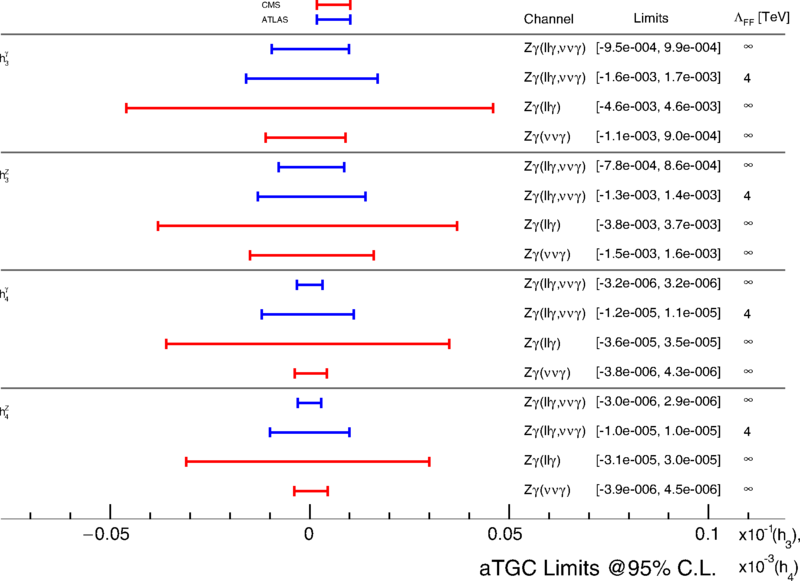
\includegraphics[width=\textwidth]{Figures/lhc_8tev_atgc_1dlimits.png}
    \caption{
      1D $h_{i}^{V}$ exclusion limits from the ATLAS and CMS experiments at the LHC based on 20 \fbinv\ of $\sqrt{s} = 8$ TeV
      $pp$ collision data. $Z\gamma(ll\gamma)$ indicates a combination of $Z(e^\mathrm{+}e^\mathrm{-})\gamma$ and $Z(\mu^\mathrm{+}\mu^\mathrm{-})\gamma$
      analyses; $Z\gamma(ll\gamma,\nu\nu\gamma)$ indicates a combination of these with \zinvg. The mass $\Lambda_{FF}$
      is the form factor scale; $\infty$ means no form factor was used.~\cite{ref:RevModPhys.89.035008}
    }
    \label{fig:lhc_8tev_atgc_1dlimits}
  \end{center}
\end{figure}

The most sensitive published limits on $h_{3,4}^{Z,\gamma}$ are currently derived from 36.1 \fbinv\ of 13 TeV $pp$ collision
data collected by the ATLAS detector at the LHC, analyzed exclusively in the monophoton channel, with no form factor~\cite{ref:ATLAS-CONF-2018-035}.
These are summarized in Figs.~\ref{fig:atlas_atgc_13tev_1dlimits},~\ref{fig:atlas_atgc_13tev_2dlimits}.

\begin{figure}[hbtp]
  \begin{center}
    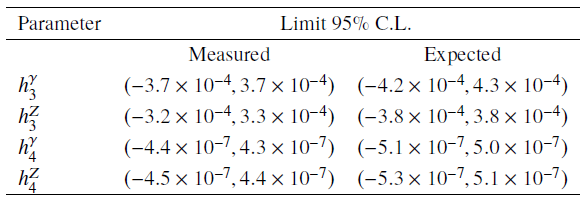
\includegraphics[width=0.8\textwidth]{Figures/atlas_atgc_13tev_1dlimits.png}
    \caption{
      1D $h_{i}^{V}$ exclusion limits from the ATLAS experiment at the LHC based on 36.1 \fbinv\ of $\sqrt{s} = 13$ TeV
      $pp$ collision data, analyzed in the monophoton channel.~\cite{ref:ATLAS-CONF-2018-035}
    }
    \label{fig:atlas_atgc_13tev_1dlimits}
  \end{center}
\end{figure}

\begin{figure}[hbtp]
  \begin{center}
    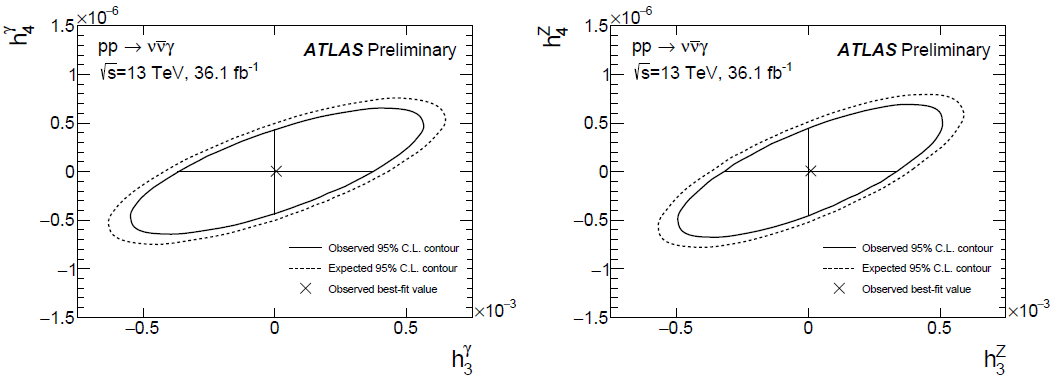
\includegraphics[width=\textwidth]{Figures/atlas_atgc_13tev_2dlimits.png}
    \caption{
      2D $h_{i}^{V}$ exclusion contours from the ATLAS experiment at the LHC based on 36.1 \fbinv\ of $\sqrt{s} = 13$ TeV
      $pp$ collision data, analyzed in the monophoton channel.~\cite{ref:ATLAS-CONF-2018-035}
    }
    \label{fig:atlas_atgc_13tev_2dlimits}
  \end{center}
\end{figure}

None of these analyses report any significant deviation from SM predictions.

\section{Dark matter EFT and simplified models} \label{sec:introduction_dm}
One example of a phenomenon with no apparent SM explanation is ``dark matter''. On cosmological scales there appears to be an abundance of massive
matter with no interactions of any sort other than its gravitational pull~\cite{ref:s41550-017-0059}.
No SM particle is predicted to exhibit this behavior, and this has spurred the development of BSM theories aiming to account for it~\cite{ref:j.physrep.2004.08.031, ref:annurev.nucl.54.070103.181244, ref:S1062798717000783}.

The great diversity of theories has motivated the analysis of general models that can potentially constrain a wide variety of specific theories simultaneously.
If DM is particulate in nature, it apparently has a substantial mass, interacts very weakly with SM particles, and is stable on cosmological timescales,
and the models we consider include a BSM particle satisfying these criteria.
All the massive, stable particles in the SM are fermionic, and these models similarly describe a fermionic DM candidate. Otherwise, the new physics
content of these models is kept to a minimum, as sufficiently large deviations from SM predictions would have been detected by now.

One model we examine describes a direct coupling between DM and the neutral EWK vector bosons \PZ\ and \Pgamma~\cite{ref:PhysRevD.89.056011}. The model does not fully specify
the nature of the proposed particle and its SM interactions, but rather only predicts the most dominant potential signature of new physics,
by adding a handful of new operator terms to the SM Lagrangian. Any operator has a ``mass dimension'', denoted in powers of GeV. The SM Lagrangian has
a mass dimension of 4, and any operator term added to it has to have this same mass dimension for the expression to be coherent.
Additional particle interactions in an operator term tend to raise the mass dimension. If an operator describes an especially intricate interaction,
the overall term must be multiplied by an extra factor of $\frac{1}{\Lambda^{n}}$ to maintain an overall mass dimension of 4, where $\Lambda$ is some mass
scale in GeV and $n$ is a positive number.

Operator terms with nonzero powers of $\frac{1}{\Lambda}$ tend to have their interactions suppressed for interaction energies much
smaller than $\Lambda$, and so $\Lambda$ is called the suppression scale. More complicated terms, multiplied by higher powers of $\frac{1}{\Lambda}$,
are expected to have effects that become apparent at higher energy scales, so a model that only incorporates simpler terms is expected to
lose predictive validity as $\Lambda$ is approached~\cite{ref:j.aop.2013.04.016}. A model that only adds the simplest possible terms with powers of
$\frac{1}{\Lambda}$ greater than zero, with predictive validity only up to energies below $\Lambda$, is called an EFT.

The DM-EWK EFT described in~\cite{ref:PhysRevD.89.056011} adds four dimension-7 interaction terms to the SM Lagrangian, which therefore carry factors of $\frac{1}{\Lambda}$
raised to the third power. The mass $m_\mathrm{DM}$ of the new DM particle is a free parameter of the model, along with two constants $k_1$ and $k_2$ controlling
the relative strengths of the DM-\PZ\ and DM-\Pgamma\ couplings.
Fig.~\ref{fig:dm_diagrams} illustrates the dominant contribution of this interaction to monophoton yields. Since the DM
particle only interacts with the \PZ\ and \Pgamma, and this interaction is suppressed by $\frac{1}{\Lambda^{3}}$, the outgoing DM is not expected to interact at all
with any detector apparatus.

\begin{figure}[hbtp]
  \begin{center}
    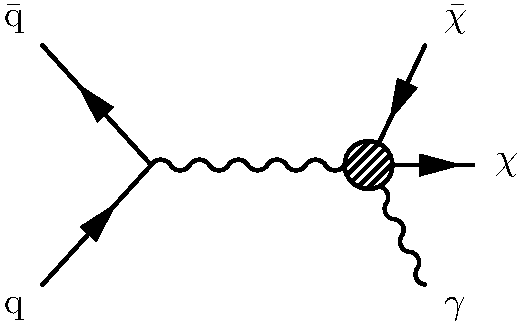
\includegraphics[width=0.42\textwidth]{Figures/dmewk.pdf}
    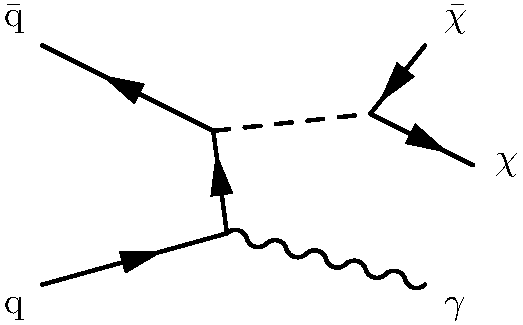
\includegraphics[width=0.42\textwidth]{Figures/dm.pdf}
    \caption{
      Leading order Feynman diagrams for monophoton processes in a DM-EWK EFT (left) and in DM simplified models (right).
      The intermediate boson in the EFT diagram can be a \PZ\ or \Pgamma. The dotted line in the DM simplified model diagram
      stands for the DM-quark mediator.
    }
    \label{fig:dm_diagrams}
  \end{center}
\end{figure}

Since the DM emerges directly from an EWK boson, this EFT is limited in the sort of dynamics it can describe. So-called simplified models of DM add
a new mediating boson between the DM and SM fermions~\cite{ref:1507.00966}, which more typically characterizes the fermion interactions that we know
from the SM. We examine models
in which the mediator has either exclusively vector or exclusively axial-vector couplings to DM and also to SM quarks, independently
of quark flavor. The free parameters of this model include
the DM mass $m_\mathrm{DM}$, the mediator mass $M_\mathrm{med}$, the DM-mediator coupling $g_\mathrm{DM}$ and the DM-quark coupling $g_\mathrm{q}$.
The leading Feynman diagrams for monophoton production are shown in Fig.~\ref{fig:dm_diagrams}. The mediators are typically chosen to be quite massive,
which suppresses the likelihood of DM-quark interactions, and the DM is not expected to interact with detector elements as it escapes.

\subsection{Previous searches} \label{sec:introduction_dm_previous_searches}
% These models converge to an EFT in the limit that $M_\mathrm{med}$ is much larger than the $q\bar{q}$ interaction energy~\cite{ref:1603.04156}.
% Such DM-quark EFT models were the subject of monophoton searches before the adoption of DM simplified models in 2015.
% As the interaction energy increases, the EFT description breaks down for the reasons described above, and DM simplified models
% offer a replacement that retains predictive validity at the cost of some degree of generality.

\section{ADD gravitons} \label{sec:introduction_ADD}
We finally examine a model of gravitation in extra dimensions originally proposed by Arkani-Hamed, Dimoupolos, and Dvali (ADD)~\cite{ref:S0370-2693(98)00466-3}.
Gravity typically affects SM particles much, much less than the other fundamental interactions. The weakness of gravity
is often expressed in terms of a fundmental mass scale $M_\mathrm{Pl}$ (\textasciitilde$10^{19}$ GeV), which is
many orders of magnitude larger than the masses of the EWK bosons (\textasciitilde$10^{2}$ GeV). Particle-level gravitational interactions
are correspondingly sharply suppressed. The proposed boson of gravitation, the graviton, has yet to be detected and is not part of the SM.

Everyday experience indicates that there are 3 dimensions of space and 1 dimension of time, and the SM assumes this to be true.
The ADD model begins with the observation that, if there are $n$ extra spatial dimensions beyond the usual 3,
we might not be able to directly perceive them if all the SM particles are confined by some as-yet-unspecified
mechanism to a 3+1-dimensional subspace (the ``brane'') of the full $n$+3+1-dimensional spacetime (the ``bulk'').
Gravitons, assuming they exist, might in contrast be able to propagate freely throughout the bulk.

Gravitation in the bulk would be characterized by its own mass scale $M_\mathrm{D}$ distinct from the mass scale $M_\mathrm{Pl}$ that
characterizes gravitation as perceived by particles confined to the brane. If the extra dimensions are not extended infinitely like the
dimensions of common experience, but rather ``compactified'' into a finite volume of characteristic radius $R$, then for a sufficiently mild
energy density in the vicinity of the brane, $M_\mathrm{Pl}^{2} \approx M_\mathrm{D}^{n+2} R^{n}$~\cite{ref:S0370-2693(98)00466-3, ref:S0550-3213(99)00044-9}.
For a modest number of extra dimensions (e.g. $3 \leq n \leq 6$), the observed large value of $M_\mathrm{Pl}$ could then really
be a consequence of a large value for $R$, while the gravitational scale $M_\mathrm{D}$ could be closer to or even
fundamentally the same thing as the EWK scale. In light of this possibility, ADD model predictions are typically examined for values of $M_\mathrm{D}$
in the vicinity of 1 TeV.

Ref.~\cite{ref:S0550-3213(99)00044-9} calculates the cross sections for a variety of graviton production scenarios, using a low-energy EFT
approximation in which $M_{D}$ serves as the suppression scale. At higher energies the specific details of the geometry of the extra dimensions,
and phenomena uniquely predicted by a full quantum theory of gravitation, would start to become apparent. These are both unknown, so the EFT
is appropriately silent on the outcome of scattering events with energies above $M_{D}$.

The ratio $M_\mathrm{Pl} / M_\mathrm{D}$ essentially expresses the wide range of kinematic possibilities that open up for gravitons with the addition
of extra dimensions. After summing over all of these possibilities, the resulting
cross section is high enough for graviton production to be probed with existing collider experiments.
Gravitons couple to every SM particle, although the coupling is still sufficiently weak that an emitted graviton will generally not interact with a detector element.
This results in a monophoton signature if it is emitted opposite a photon, as illustrated in Fig.~\ref{fig:add_diagram}.

\begin{figure}[hbtp]
  \begin{center}
    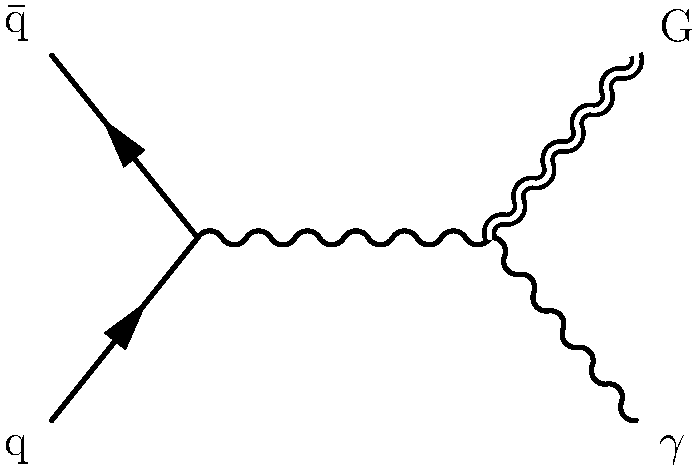
\includegraphics[width=0.42\textwidth]{Figures/add.pdf}
    \caption{
      Diagram illustrating ADD graviton emission resulting in a monophoton signature.
    }
    \label{fig:add_diagram}
  \end{center}
\end{figure}

\subsection{Previous searches} \label{sec:introduction_ADD_previous_searches}

\chapter{The CMS experiment and the LHC} \label{chap:LHCCMS}
\section{The LHC} \label{sec:LHCCMS_LHC}
\subsection{Proton acceleration} \label{sec:LHCCMS_LHC_proton_acceleration}
\subsection{Magnets and beam halo} \label{sec:LHCCMS_LHC_magnets_beam_halo}
Beam halo is an important component of the monophoton analysis and it comes from here.
\section{The CMS experiment} \label{sec:LHCCMS_CMS}
\subsection{Coordinate system} \label{sec:LHCCMS_CMS_coordinates}
\subsection{Superconducting solenoid and silicon tracking system} \label{sec:LHCCMS_CMS_magnet_tracker}
\subsection{Electromagnetic calorimeter} \label{sec:LHCCMS_CMS_ECAL}
The discussion of APDs segues into an introduction to ECAL spikes.
\subsection{Hadronic calorimeter} \label{sec:LHCCMS_CMS_HCAL}
\subsection{Muon systems} \label{sec:LHCCMS_CMS_muon}
\subsection{Trigger system} \label{sec:LHCCMS_CMS_trigger}
\subsection{Luminosity measurement} \label{sec:LHCCMS_CMS_lumi}

\chapter{Simulation} \label{chap:simulation}
\section{Hard process generation} \label{sec:simulation_hard_process}
\section{Parton distribution functions} \label{sec:simulation_pdf}
\section{Parton showering and hadronization} \label{sec:simulation_parton_shower_hadronization}
\section{Pileup simulation} \label{sec:simulation_pileup}
\section{Detector simulation} \label{sec:simulation_detector}

\chapter{Object reconstruction and selection} \label{chap:reconstruction}
\section{The particle-flow algorithm} \label{sec:reconstruction_particle_flow}
\section{Photons and electrons} \label{sec:reconstruction_egamma}
\section{Muons} \label{sec:reconstruction_muons}
\section{Jets and missing transverse momentum} \label{sec:reconstruction_jetmet}
A discussion of jets is followed by a definition of \MET\ and Type-1 \MET\ corrections.
\section{Primary vertex} \label{sec:reconstruction_pv}

\chapter{Event selection} \label{chap:event_selection}
\section{The monophoton signature and background sources} \label{sec:event_selection_backgrounds}
Summarize how each of the physics processes being analyzed exhibits a monophoton signature.
List the sources of background in the monophoton channel, to justify the ensuing cuts.
\section{Trigger and \texorpdfstring{\MET}{pTmiss} filters} \label{sec:event_selection_trigger_METfilters}
Trigger path, trigger efficiency

\MET\ filters
\section{Photon} \label{sec:event_selection_photon}
Photon kinematic cuts; Photon ID defintion, efficiency; Spike and beam halo cuts; phoET-dependent cross section corrections
\section{Missing transverse momentum} \label{sec:event_selection_MET}
$\MET > 170$ GeV; $\Delta\phi(\Pgamma,\vecMET) > 0.5$; $\mathrm{min}\Delta\phi(\mathrm{jets},\vecMET) > 0.5$;
$\ETgamma/\MET < 1.4$
\section{Lepton vetoes} \label{sec:event_selection_lepveto}
Electron selection; Muon selection
\section{Single electron control region} \label{sec:event_selection_monoele}
\section{Single muon control region} \label{sec:event_selection_monomu}
\section{Dielectron control region} \label{sec:event_selection_diele}
\section{Dimuon control region} \label{sec:event_selection_dimu}

\chapter{Background estimation} \label{chap:background_estimation}
For each component, describe its estimation and uncertainties
\section{Simulated backgrounds} \label{sec:background_estimation_simulated}
\section{Electron faking photon} \label{sec:background_estimation_elefake}
\section{Jet faking photon} \label{sec:background_estimation_jetfake}
\section{Spikes} \label{sec:background_estimation_spikes}
\section{Beam halo} \label{sec:background_estimation_halo}
\section{Transfer factors} \label{sec:background_estimation_transfer_factors}
\section{Likelihood function} \label{sec:background_estimation_likelihood}

\chapter{Results} \label{chap:results}
\section{\texorpdfstring{\zinvg}{Z(νν)γ} cross section} \label{sec:results_znng_xsec}
\section{aTGC limits} \label{sec:results_aTGC}
\section{DM simplified model limits} \label{sec:results_DM}
\section{ADD limits} \label{sec:results_ADD}

\chapter{Conclusions} \label{chap:conclusions}
\section{Summary} \label{sec:conclusions_summary}
\section{Outlook} \label{sec:conclusions_outlook}

\bibliographystyle{utcaps}
\bibliography{references}
\end{document}
